\documentclass{standalone}
\usepackage{tikz}
\usepackage{tabularx}
\usepackage{colortbl}
\usepackage{booktabs}

\begin{document}
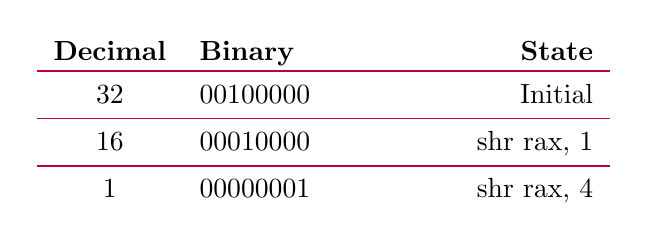
\begin{tikzpicture}

\node (tbl) {
\begin{tabularx}{.6\textwidth}{cXrcc}
\arrayrulecolor{purple}
\textbf{Decimal} & \textbf{Binary} & \textbf{State} \\
\toprule
32 & 00100000 & Initial \\ 
\midrule
16 & 00010000 & shr rax, 1 \\
\midrule
1 & 00000001 & shr rax, 4 \\
\end{tabularx}
};

\end{tikzpicture}
\end{document}